\documentclass[11pt]{article}
\usepackage[T1]{fontenc}
\usepackage[left=12mm,
right=12mm,top=1.5in,
bottom=1.5in]{geometry}
\usepackage{mathtools}
\usepackage{cancel}
\usepackage{graphicx}
\usepackage{grffile}
\graphicspath{{/home/piotr/Documents/scientific-computing/list04/exercise5/plots/}}
\DeclareUnicodeCharacter{2212}{-}
\begin{document}
\title{Zadanie 7 Lista 4}
\author{Piotr Popis, 245162}
\maketitle
\centering

\begin{flushleft}
\section{Zadanie 1}
\subsection{Opis problemu}
Celem zadania jest implementacja funkcji obliczającej ilorazy różnicowe. Danymi wejściowymi są:
\begin{center}
x- wektor długości n+ 1 zawierający węzły $x_0, . . . , x_n$  $x[1]=x_0,...,x[n+1]=x_n$\\
f– wektor długości n+1 zawierający wartości interpolowanejfunkcji w węzłach $f(x_0), . . . , f(x_n)$\\
\begin{flushleft}
Wyniki:
\end{flushleft}
fx- wektor długości $n+1$ zawierający obliczone ilorazy różnicowe\\ $fx[1]=f[x_0]$,\\$fx[2]=f[x_0, x_1],...,fx[n]=f[x_0, . . . , x_{n−1}],fx[n+1]=f[x_0, . . . , x_n].$
\begin{flushleft}
Addytywnym utrudnieniem jest restrykcja użycia tablicy dwuwymiarowej, czyli macierzy.
\end{flushleft}
\end{center}
\subsection{Rozwiązanie}
Ilorazem różnicowym n- tego rzędu funkcji $f:X\longrightarrow Y$ w punktach $x_0, ..., x_n \epsilon X$ nazywamy funkcję:\\
\begin{center}
$f(x_0,...,x_n) := \Sigma^n_i\dfrac{f(x_i)}{\Pi^n_j(x_i-x_j)}$
\end{center}
W celu realizacji zadania, czyli uniknięcia wykorzystania macierzy skorzystamy z zależności rekurencyjnej:\\
1.$i=0$\\
\quad$f[x_0]=f(x_0)$\\
2.$i=1$\\
\quad$f[x_0,x_1]=\dfrac{f(x_1)-f(x_0)}{x_1-x_0}$\\
3.$i=n$\\
\quad$f[x_0,...,x_n]=
\dfrac{f(x_1,...,x_n)-f(x_0,...,x_{n-1})}{x_n-x_0}$\\
Znając węzły $x_n$ i wartości funkcji f($x_n$), można utworzyć dwuwymiarową tablicę ilorazów różnicowych. Jednak algorytm można zoopytmalizować, ponieważ wystarczy użyć tablicy jednowymiarowej $w$ do zapamiętywania dwóch poprzednich wartości(tablicę aktualizujemy od dołu do góry i od lewej do prawej). Pozostałe wartości tylko i wyłącznie spowalniają nasz algorytm. Początkowymi wartości są $w_i$ są odpowiadające im f[$x_i$]. W kolejnych krokach aktualizowane jest jedno miejsce mniej.
\newpage
\section{Zadanie 2}
\subsection{Opis problemu}
Napisać funkcję obliczającą wartość wielomianu interpolacyjnego stopnia n w postaci Newtona $N_n(x)$ w punkcie x=t za pomocą algorytmu Hornera w czasie $\theta(n)$. Dane wejściowe:\\
\begin{center}
x– wektor długości n+ 1 zawierający węzły $x_0, ...,x_n$\\$x[1]=x0,...,x[n+1]=x_n$\\
fx– wektor długości n+ 1 zawierający ilorazy  różnicowe \\$fx[1]=f[x_0]$,\\
$fx[2]=f[x_0, x_1],...,fx[n]=f[x_0, . . . , x_{n−1}],fx[n+1]=f[x_0, . . . , x_n]$
\end{center}
\begin{flushleft}
Wyniki:
\begin{center}
a – wektor długości n+ 1 zawierający obliczone współczynniki postaci naturalnej\\
$a[1]=a_0$,\\
$a[2]=a_1,...,a[n]
=a_{n−1},a[n+1]=a_n$.\\
\end{center}
\end{flushleft}
\subsection{Rozwiązanie}
W celu wyznaczenia wartości wielomianu interpolacyjnego stopnia n w postaci Newton'a $N_n(x)$ w punkcie $x=t$ zaimplementowano uogólniony schemat Hornera.\\
\begin{center}
$N_n(x)=\Sigma^k_{i=0}c_i\Pi^{i-1}_{j=0}(x-x_j)$
\end{center}
Wartość wielomianu przyjmowana w danym punkcie t obliczamy, kosztystając z:\\
\begin{center}$w(x)=(x-t)\cdot q(z)\cdot w(t)$\end{center}
Można też śmiało stwierdzić, iż metoda Newton'a jest trudniejsza w impementacji niż np metoda Lagrange'a i wymaga większej ilości oddzielnych kroków. Jest jednak znacznie lepiej uwarunkowana nmerycznie.W metodzie najpierw wzynaczane są odpowiednie ilorazy różnicowe, a dopiero później z ich użyciem- interpolowa funkcja.\\
Algorytm zaczynamy od przypisania do zmiennej nt konkretnego wektora ilorazów różnicowych. W kolejnych krokach od n-1 zwiększamy wartość wektora pomnożoną przez różnicę wartości węzła i weilomianu t. Otrzymujemy:\\
\begin{center}
$nt=f_x(i)+nt\cdot (t-\omega[i])$, gdzie $f_x$ jest wektorem ilorazów różnicowych.\\
\end{center}
Algorytm działa w czasie liniowym.
\newpage
\section{Zadanie 3}
\subsection{Opis Problemu}
Celem zadania jest kreacja funkcji obliczającej współczynniki postaci naturalnej wielomianu interpolacyjnego znając współczynniki wielomianu interpolacyjnnego w postaci Newton'a $c_0$ = f[$x_0$], $c_1$ = $f[x_0,x_1]$, $c_2$= $f[x_0, x_1, x_2],. . .,cn=f[x_0, . . . , x_n]$ (ilorazy różnicowe) oraz węzły $ x_0, x_2, . . . , x_n $ działającą w czasie $\theta(n^2)$. Dane wejściowe:\\
\begin{center}
x– wektor długości $n+ 1 $ zawierający węzły $x_0, . . . , x_n x[1]=x_0,...,x[n+1]=x_n$ \\
fx– wektor długości n+ 1 zawierający ilorazy różnicowe $fx[1]=f[x_0],fx[2]=f[x_0, x_1],...,fx[n]=f[x0, . . . , x_{n−1}],fx[n+1]=f[x0, . . . , x_n]$\\
\begin{flushleft}
Wyniki:\\
\end{flushleft}
a– wektor długości $n+ 1 $ zawierający obliczone współczynniki postaci naturalnej\\
$a[1]=a_0$,\\
$a[2]=a_...,a[n]=a_{n−1},a[n+1]=a_n$
\end{center}
\bigskip
\subsection{Rozwiązanie}
\bigskip
Korzystając z faktu, iż współczynnik sąsiadujący z $x^k$ to f[$x_0,x_1,...,x_k$], czyli $c_n$ przy najwyżej potędze wielomianu w postaci Newton'a. Ponownie wykorzystujemy ugólnienie schematu Hornera, a następnie z wzoru na postać Newton'a podanego na  wykładzie: \\
\begin{center}
\bigskip
$p(x) = \Sigma^n_{k=0} f[x_0,...,x_k] \Pi^{k-1}_{j=0}(x-x_j)$\\
\bigskip
\end{center}
Wielomian posiada współczynniki przy odpowiadających im potęgach $a_0,a_1,...,a_k$, gdzie współczynnik $a_k$ leży przy największej potędze. Dokonujemy mnożenia danego wielomianu począwszy od jego ostatnich potęg. W każdym kroku mnożemy nasz  wielomian przez dwumian $(x-x_{n-1})$. Ostateczny wielomian wynikowy będzie zaprezentwoany jako prosty wektor współczynników analagoiczny do wektora wejściowego. W wyniku wykonanych mnożeń otrzymujemy postać wynikową wielomianu, którego współczynniki wynoszą kolejno $a_k,a_{k-1},..,a_0$. Aby wynik był postaci $a_0+a_1x+a_x^2+...+a_nx^n$ musimy dokonać również przestawienia. Całkowita złożoność obliczeniowa wynosi $\theta(n^2)$, ponieważ złożoność obliczeniowa schmeatu Horner;a wynosi $\theta(n)$ oraz mnożenie wielomianów również $\theta(n)$
\newpage
\section{Zadanie 4}
\subsection{Opis Problemu}
Celem zadania jest utworzenie funkcji, która zinterpoluje zadaną funkcję f(x) w przedziale [a,b] za pomocą wielominau interpolacyjnego stopnia n w postaci Newton'a, a następnie narysuje wielomian interpolacyjny i funkcję interpolową. Wykorzystać Plots lub PyPlot lub Gadfly do narysowania grafów.\\
\quad W interpolacji użyć węzłów równoodległych, \\
\bigskip
\quad\quad$x_k=a+k\cdot h$,\\
\quad\quad $h =\dfrac{b-a}{n}, k = 0,1...,n$\\
W zadaniu należy nie wyznaczać jawnej postaci wielomianu interpolacyjnego. Należy skorzystać z funkcji zaimplementowanych w zadaniu 1 oraz zadaniu 2 odpowiednio iloryRzonicowe i warNewton. Dane wejściowe:\\
\begin{center}
f– funkcja f(x) zadana jako anonimowa funkcja,\\
a,b– przedział interpolacji, 
\\n– stopień wielomianu interpolacyjnego
\begin{flushleft}
Wyniki:
\end{flushleft}
-funkcja rysuje wielomian interpolacyjny i interpolowaną funkcję w przedziale[a, b]
\end{center}
\bigskip
\subsection{Rozwiązanie}
\bigskip
Pierwszym schodem jest wyznaczenie równoodległch węzłów i obliczenie odległosci h między nimi z wzoru
\bigskip
\begin{center}
$h=\dfrac{b-a}{n}$.\\
\end{center} 
\bigskip
 Kolejnym etapem jest wyznaczenie wartości zadanej funkcji w wyznaczonych węzłach.\\ Następnie korzystając z funkcji zaimplementowanej w sekcji Zadanie 1 - ilorazyRoznicowe, tablic z węzłami i wartościami funkcji wyznaczenie wektora ilorazów różnicowych.\\ Przedostatni krok to wyznaczenie wartości funkcji interpolowanej i wielomianu interpolacyjnego w s równoodległych punktach na zadanym przedziale .\\ Ostatni etap to rysunek wykorzystując pakiet Plots.\\
\bigskip
 W pliku tekst znajdują się testy do powyższych funkcji. Wszystkie powyższe funkcje zostały umieszczone w wspólnym module - $functions$
 
\newpage
\section{Zadanie 5}
\subsection{Opis Problemu}
\subsubsection{a) $ e^x,[0,1],n= 5,10,15,$}
\subsubsection{b) $ x^2sin(x),[−1,1],n= 5,10,15$}
\subsection{Rozwiązanie}
W celu rozwiązania zadania należy przetestować zaimplementowaną w Zadaniu 4 funkcję i narysować wykresy dla zadanych przykładów
\subsection{Wyniki}
\subsubsection{a) $ e^x,[0,1],n= 5,10,15,$}
\begin{figure}[htbp]
\centering
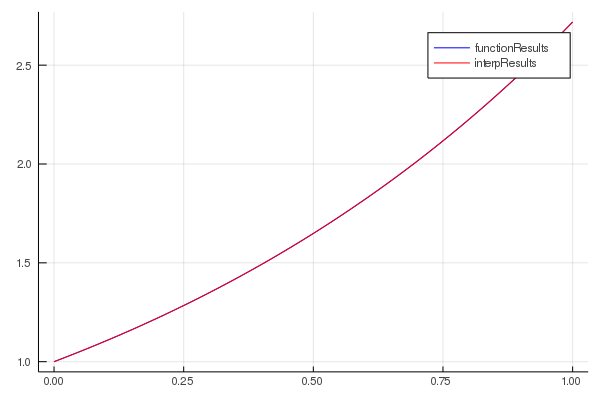
\includegraphics[scale=.4]{PLOT:0.0-1.0-5.png}
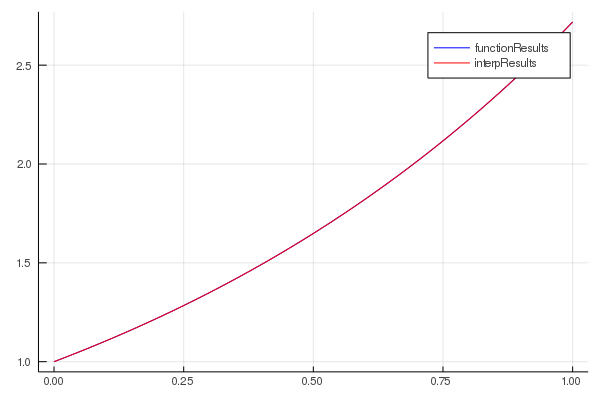
\includegraphics[scale=.4]{PLOT:0.0-1.0-10.png}
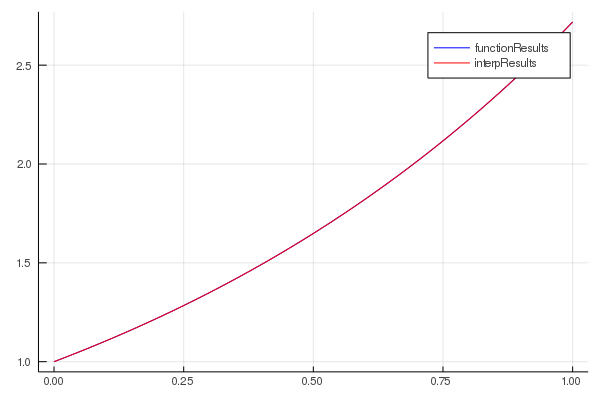
\includegraphics[scale=.4]{PLOT:0.0-1.0-15.png}
\end{figure}
\newpage
\subsubsection{b) $ x^2sin(x),[−1,1],n= 5,10,15$}
\begin{figure}[htbp]
\centering
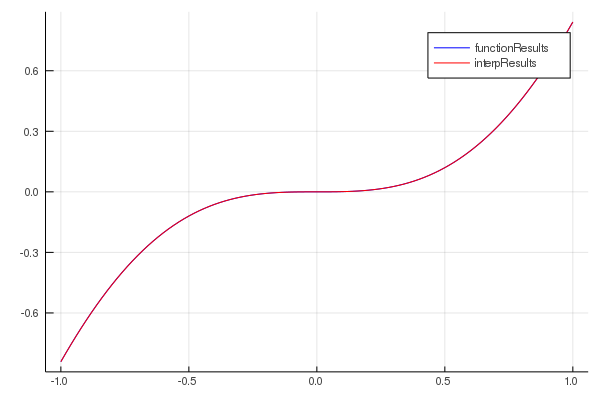
\includegraphics[scale=.4]{PLOT:-1.0-1.0-5.png}
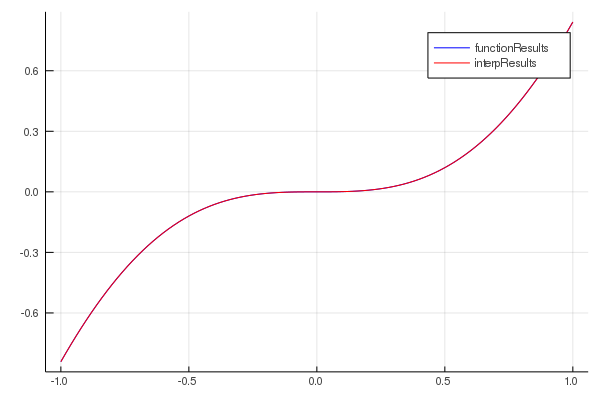
\includegraphics[scale=.4]{PLOT:-1.0-1.0-10.png}
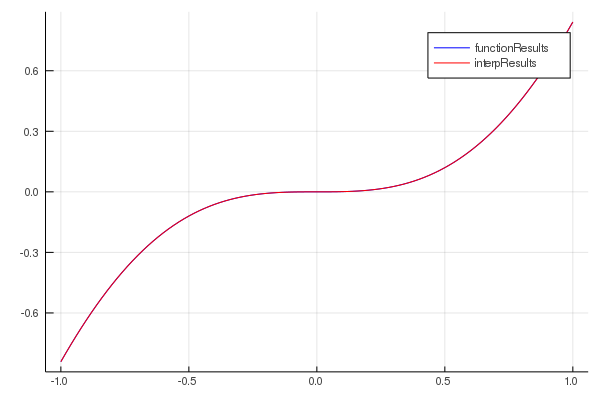
\includegraphics[scale=.4]{PLOT:-1.0-1.0-15.png}
\end{figure}

\subsection{Wnioski}
xxxxxxxxxx


\end{flushleft}
\end{document}